% Copyright Aidan Randle-Conde 2007-2014
% http://www.aidansean.com/phd_notes
% Anyone is free to download, redistribute, edit and use these notes and the source tex files with the following restrictions:
% This 
%  This message is included in the tex source files.
%  Aidan Randle-Conde is credited as the author.
%  Images are correctly credited to their respective authors, as outlined in the references.
%  No part of these notes may be used for commercial purposes.

\chapter{Compton scattering}

Feynmann diagrams for the process $e\gamma \to e\gamma$ are:

\begin{figure}[!htb]
  \begin{center}
    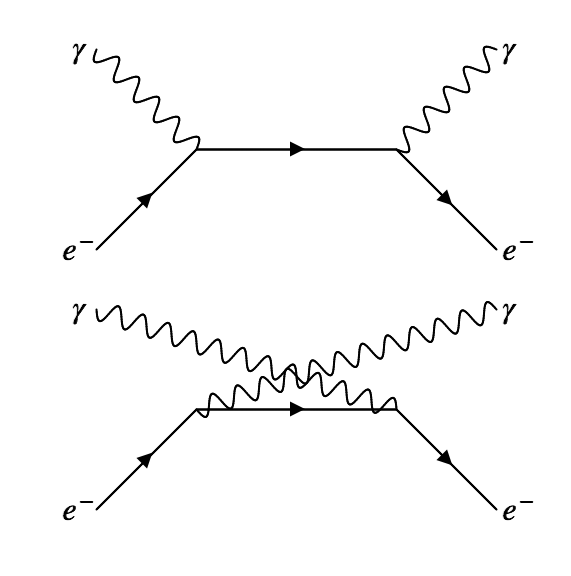
\includegraphics[width=0.5\textwidth]{images/web_feynman/image_36.png}
    \caption[Compton scattering processes]{Compton scattering processes ($e\gamma\to e\gamma$).}
    \label{fig:ch11_Compton}
  \end{center}
\end{figure}

These processes are closely related to $e^+e^-$ annihilation:

\begin{figure}[!htb]
  \begin{center}
    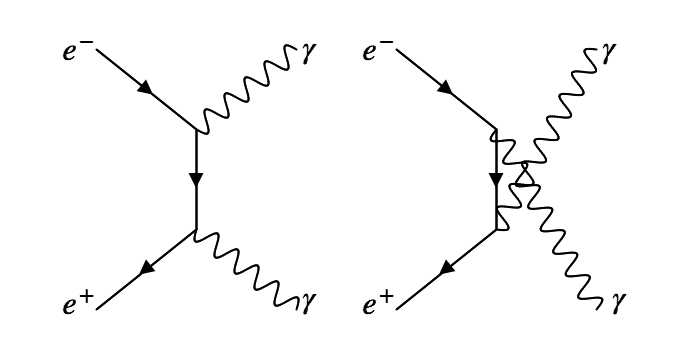
\includegraphics[width=0.75\textwidth]{images/web_feynman/image_37.png}
    \caption[$e^+e^-$ annihilation processes]{$e^+e^-$ annihilation processes.}
    \label{fig:ch11_EpemToGGc}
  \end{center}
\end{figure}

Calculating the cross-section for Compton scattering is also useful for deriving the cross-section for the QCD Compton process.

\begin{figure}[!htb]
  \begin{center}
    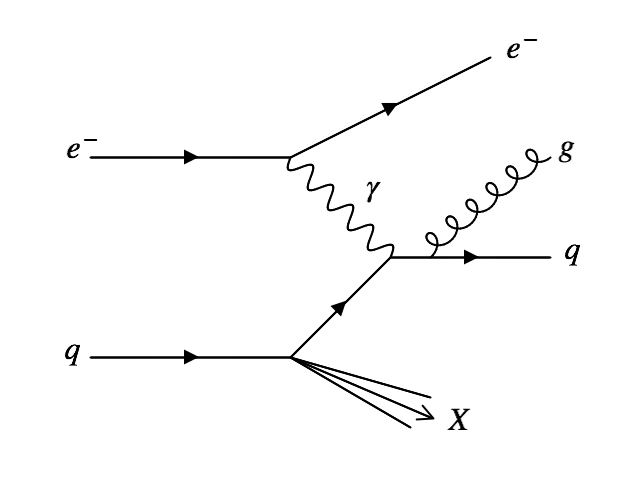
\includegraphics[width=0.75\textwidth]{images/web_feynman/image_38.png}
    \caption[QCD Compton process]{QCD Compton process ($\gamma q \to qg$).}
    \label{fig:ch11_GammaQToGQ}
  \end{center}
\end{figure}

Boson-gluon fusion (BGF):

\begin{figure}[!htb]
  \begin{center}
    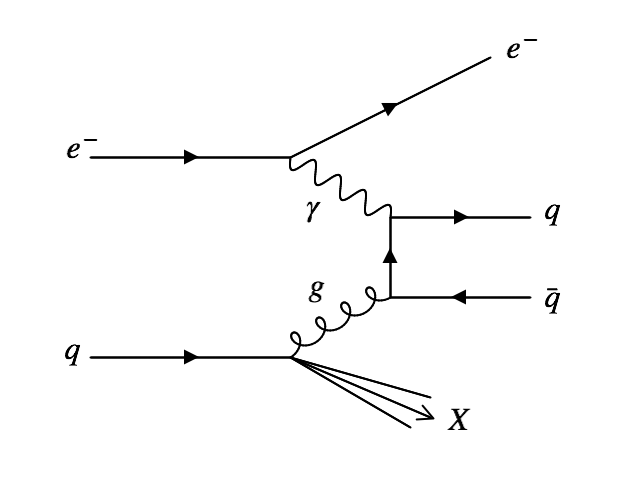
\includegraphics[width=0.75\textwidth]{images/web_feynman/image_39.png}
    \caption[Boson gluon fusion process]{Boson gluon fusion process ($\gamma q \to q\bar{q}$).}
    \label{fig:ch11_GammaQToQQ}
  \end{center}
\end{figure}

The above diagrams cause structure functions to evole with $Q^2$ of the probe (in this case the photon).

\begin{figure}[!htb]
  \begin{center}
    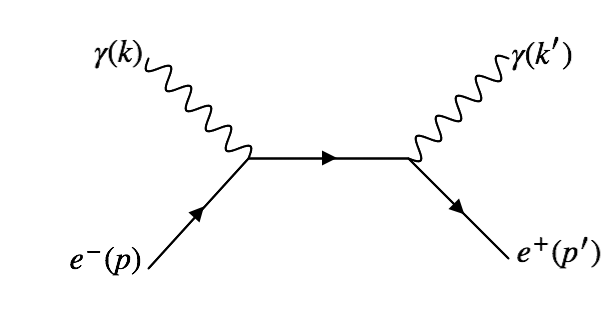
\includegraphics[width=0.75\textwidth]{images/web_feynman/image_40.png}
    \caption[$s$ channel Compton scattering]{$s$ channel Compton scattering.}
    \label{fig:ch11_ComptonSChannel}
  \end{center}
\end{figure}

\begin{eqnarray*}
  s & = & (k + p)^2  \\
  t & = & (k - k')^2 \\
  u & = & (k - p')^2
\end{eqnarray*}

This is a double scattering process.  Recall:

\begin{eqnarray*}
  T_{fi} & = & -i\int\mathrm{d}^4x_1\int\mathrm{d}^4x_2\phi^{\star}(2)V(2)G_0(2,1)V(1)\phi(1) \\
  & = & -i\int\mathrm{d}^4x_1\int\mathrm{d}^4x_2\left(\e\right)\bar{u}\e^{ip'x_2}\e^{ik'x_2}\epsilon^{\star}_{\nu}\gamma^{\nu}\frac{1}{\left(2\pi\right)^4}\e^{-i(p + k)(x_2 - x_1)}\\
  &   & \times i\frac{\not{p} + \not{k} + m}{(p + k)^2 - m^2}\left(-\e\right)\epsilon_{\mu}\e^{-ikx_2}\gamma^{\mu}u\e^{-ipx_1}
\end{eqnarray*}

In the above expression the integration $\int\mathrm{d}^4x\e^{-i(p + k)(x_2 - x_1)}$ gives $\delta^4(x_2 - x_1)$, so $x_2$ and $x_1$ can be replaced with a dummy variable $x$.  The exponential in terms of the four-momentum, combined with other terms gives the volume and time and the number of state vectors as before.  Therefore $T_{fi}$ can be more simply expressed as:

\[
  T_{fi} = -i\bar{u}(p')(-\e)\epsilon^{\star}_{\nu}\gamma^{\nu}
           \left(\frac{\not{p} + \not{k} + m}{(p + k)^2 - m^2}\right)
           (-\e)\epsilon_{\mu}\gamma^{\mu}u(p)
\]

Assume $m \to 0$, then:

\begin{eqnarray*}
  T_{fi}     & = & -\frac{i\e^2}{s}\bar{u}(p')\epsilon^{\star}_{\nu}\gamma^{\nu}\left(\not{p} + \not{k}\right)\epsilon_{\mu}\gamma^{\mu}u(p) \\
  |T_{fi}|^2 & = & \frac{\e^4}{s^2}\left(\epsilon^{\star}_{\mu'}\epsilon_{\nu'}\epsilon^{\star}_{\nu}\epsilon_{\mu}\bar{u}(p)\gamma^{\mu'}\left(\not{p} + \not{k}\right)\gamma^{\nu'}u(p')\bar{u}(p')\gamma^{\nu}\left(\not{p} + \not{k}\right)\gamma^{\mu}u(p)\right)
\end{eqnarray*}

This must be summed over initial and final spin states and averaged over the initial spin states, $1/4$.  For the sum over the initial photon polarisation states:

\[
  \sum\epsilon^{\star}_{\mu}\epsilon_{\mu'} = -g_{\mu\mu'}
\]

The sum over the initial and final electron states is again performed by using the completeness relation for $u\bar{u}$ as in $e\mu$ scattering:

\begin{eqnarray*}
  |T_{fi}|^2 & = & \frac{\e^4}{4s^2}g_{\mu\mu'}g_{\nu\nu'}Tr[\left(\not{p}' + m\right)\gamma^{\mu'}\left(\not{p} + \not{k}\right)\gamma^{\nu'}\left(\not{p} + m\right)\gamma^{\nu}\left(\not{p} + \not{k}\right)\gamma^{\mu}] \\
  & = & \frac{\e^4}{4s^2}Tr[\gamma^{\mu}\not{p}'\gamma_{\mu}\left(\not{p} + \not{k}\right)\gamma_{\nu}\not{p}\gamma^{\nu}\left(\not{p} + \not{k}\right)] \\
  & = & \frac{\e^4}{s^2}Tr[\not{p}'\left(\not{p} + \not{k}\right) \not{p}\left(\not{p} + \not{k}\right)] \\
  & = & \frac{\e^4}{s^2}Tr[\not{p}'\not{k}\not{p}\not{k}] \\
  \textrm{where } \not{p}'\not{p} & = & m^2_{e} \textrm{ terms have been neglected} \\
  |T_{fi}|^2 & = & \frac{4\e^4}{s^2}\left((p'\cdot k)(p\cdot k) - (p'\cdot p)(k\cdot k) + (p'\cdot k)(k\cdot P)\right) \\
  k\cdot k & = & 0 \textrm{ as the photon is massless} \\
  \textrm{So } |T_{fi}|^2 & = & \frac{2\e^4}{s^2}\left(2(p'\cdot k)2(p\cdot k)\right) \\
  & = & \frac{2\e^4}{s^2}(-us) \\
  & = & -2\e^4\left(\frac{u}{s}\right)
\end{eqnarray*}

For the second diagram:

\begin{figure}[!htb]
  \begin{center}
    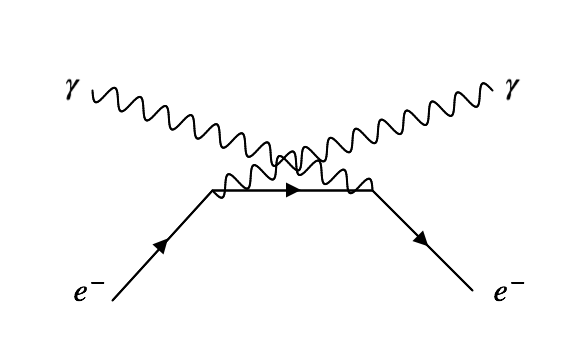
\includegraphics[width=0.75\textwidth]{images/web_feynman/image_41.png}
    \caption[$u$ channel Compton scattering]{$u$ channel Compton scattering.}
    \label{fig:ch11_ComptonUChannel}
  \end{center}
\end{figure}

\[
  |T_{fi}|^2 = - 2\e^4\left(\frac{s}{u}\right)
\]

For the above expressions, the matrix element is needed for the calculation of the inteference between the two diagrams.

\begin{eqnarray*}
  T_{fi} & = & -i\frac{\e^2}{u}\bar{u}(p')\epsilon_{\mu}\gamma^{\mu}\left(\not{p} - \not{k}\right)\epsilon^{\star}_{\nu}\gamma^{\nu}u(p) \\
  |T_{fi}^{I} + T_{fi}^{II}|^2 & = & |T_{fi}^{I}|^2 + |T_{fi}^{II}|^2 + T_{fi}^{\star I}T_{fi}^{II} + T_{fi}^{\star II}T_{fi}^{I} \\
  T_{fi}^{\star II}T_{fi}^{I} & = & T_{fi}^{\dagger II}T_{fi}^{I} \\
  & = & \frac{\e^2}{u}\epsilon_{\nu}\epsilon^{\star}_{\mu'}\bar{u}(p)\gamma^{\nu'}\left(\not{p} - \not{k}'\right)\gamma^{\mu'}u(p')\times\frac{\e^2}{s}\epsilon^{\star}_{\nu}\epsilon_{\mu}\bar{u}(p')\gamma^{\nu}\left(\not{p} + \not{k}\right)\gamma^{\mu}u(p) \\
  & = & \frac{\e^4}{us}\frac{1}{4}g_{\mu\mu'}g_{\nu\nu'}\stackrel{\sum\sum}{\e \textrm{ spins}}\bar{u}(p)\gamma^{\nu'}\left(\not{p} - \not{k}'\right)\gamma^{\mu'}u(p')\bar{u}(p')\gamma^{\nu}\left(\not{p} + \not{k}\right)\gamma^{\mu}u(p) \\
  & = & \frac{\e^4}{4us}Tr[\not{p}\gamma_{\nu}\left(\not{p} - \not{k}'\right)\gamma_{\mu}\not{p}'\gamma^{\nu}\left(\not{p} + \not{k}\right)\gamma^{\mu}] \\
  & = & \frac{\e^4}{4us}Tr[-2\left(\not{p} - \not{k}'\right)\gamma_{\nu}\not{p}\not{p}'\gamma^{\nu}\left(\not{p} + \not{k}\right)] \\
  \textrm{(using } \gamma_{\mu}\not{a}\not{b}\not{c}\gamma^{\mu} & = & -2\not{c}\not{b}\not{a} \textrm{)} \\
  & = & -\frac{\e^4}{2us}Tr[\not{p}\not{p'}4(p + k)(p - k')] \\
  & = & -\frac{2\e^4}{us}(p\cdot p')(p + k)(p - k') \\
  & = & 4\e^4\frac{t}{su}(p\cdot p + k\cdot p - p\cdot k' -k\cdot k') \\
  & = & 4\e^4\frac{t}{su}\left(0 + \frac{1}{2}s + \frac{1}{2}u + \frac{1}{2}t \right) \\
  & = & 2\e^4\frac{t}{su}\left(s + t + u\right) \\
  \textrm{But } s + t + u & = & 2(m_e^2 + m_{\gamma}^2) \simeq 0
\end{eqnarray*}

Thus the inteference terms for real photons scattering off nearly massless electrons does not contribute to the cross-section.  However, if the incoming photon is virtual then $s + t + u = Q^2$ and for a photon of mass $k^2 = Q^2$.

So for a real photon:

\begin{eqnarray*}
  \frac{\mathrm{d}\sigma}{\mathrm{d}\Omega} & = & \frac{1}{64\pi^2 s}2\e^4\left(\frac{-u}{s} + \frac{-s}{u}\right) \\
  & = & \frac{\alpha^2}{2s}\left(\frac{-u}{s} + \frac{-s}{u}\right) \\
  && \textrm{and for a virtual photon:} \\
  \frac{\mathrm{d}\sigma}{\mathrm{d}\Omega} & = & \frac{1}{64\pi^2s}2\e^4\left(\frac{-u}{s} + \frac{-s}{u} + \frac{2tQ^2}{su}\right)
\end{eqnarray*}

The cross-section and $|T_{fi}|^2$ for $e^+e^-$ annihilation are the same as for the above except that $s$, $t$ and $u$ are permutated.  The Compton scattering cross-section in the limits $m_e \to 0$ and $s \to \infty$ is:

\begin{eqnarray*}
  \frac{\mathrm{d}\sigma}{\mathrm{d}\Omega} & = & \frac{1}{64\pi^2s}2\e^4\left(\frac{-u}{s} + \frac{-s}{u}\right) \\
  \lim_{s\to\infty} \frac{\mathrm{d}\sigma}{\mathrm{d}\Omega} & = & \frac{1}{64\pi^2}2\e^4\left(\frac{-1}{u}\right) \\
  u & \simeq & -2p\cdot k' \\
  \frac{\mathrm{d}\sigma}{\mathrm{d}\Omega} & = & \frac{1}{64\pi^2}2\e^4\frac{-1}{-2p\cdot k'} \\
  & = & \frac{1}{64\pi^2}\frac{\e^4}{p\cdot k'}
\end{eqnarray*}

$p\cdot k'$ can be evaluated in the centre of mass system and using $E_e = \sqrt{p_e^2 + m_e^2}$:

\begin{eqnarray*}
  p\cdot k' & = & p_eE_{\gamma}\left(1 + \cos\theta + \frac{1}{2}\frac{m_e^2}{p_e^2} + \cdots \right) \\
  \Rightarrow \frac{\mathrm{d}\sigma}{\mathrm{d}\Omega} & = & \frac{1}{64\pi^2}\frac{\e^4}{\frac{s}{4}\left(1 + \cos\theta + \frac{2m_e^2}{s}\right)} \\
  \mathrm{d}\sigma & = & \frac{\alpha^2}{s}2\pi\frac{\mathrm{d}\cos\theta}{1 + \cos\theta + \frac{2m_e^2}{s}} \\
  \Rightarrow \sigma & = & \frac{2\pi\alpha^2}{s}\int\frac{\mathrm{d}l}{l} \\
  \textrm{(using } l & = & 1 + \cos\theta + \frac{2m_e^2}{s} \textrm{)} \\
  \sigma & = & \frac{2\pi\alpha^2}{s}\ln\Bigg[1 + \cos\theta + \frac{2m_e^2}{s}\Bigg]_{-1}^{1} \\
  & = & \frac{2\pi\alpha^2}{s}\ln\left(\frac{2\left(1 + \frac{m_e^2}{s}\right)}{2\frac{m_e^2}{s}}\right) \\
  & \simeq & \frac{2\pi\alpha^2}{s}\ln\left(\frac{s}{m_e}\right)
\end{eqnarray*}
